\chap{Materials and methods}
This chapter gives a brief overview of the methods used in the four studies that make up this thesis. Many of the novel concepts have been discussed in previous chapter. The purpose of this chapter is to provide complementary information on how the methods were evaluated. For a complete description, see Studies I-IV.

\sect{Study populations}
 In \textbf{Study I} the method was therefore first tested on 10 healthy volunteers (age $44\pm11$ years, 50\% female), and on two patients (age 27 and 38, both female) which had a confirmed and clinically established diagnosis of pulmonary embolism. Out of the 10 volunteers, 9 were given the same protocol as the patients. However, the last volunteer in the volunteer cohort was given an extended protocol, where the reference method was tested under several conditions other than the normal acquisitions, to isolate respiratory and cardiac motion. This required a motivated volunteer, and would not be feasible in a patient population. \textbf{Study II} was entirely focused on the methodology, and most work was made using numerical simulations and phantom images. One healthy volunteer was recruited (female, 27 years) to evaluate the method \emph{in vivo}. In addition, ECG and respiratory motion signals that were recorded in 8 healthy volunteers to be used in the numerical simulations. \textbf{Study III} was the most clinically oriented study. The purpose of the study was to study functional parameters, so patients from the clinical workflow were included on a consecutive basis. Whereas there was no stratification or other type of attempt to steer the inclusion, the final population comprised a range of different pathologies representative of what can be expected in the clinic. The population was divided into two groups chronologically. The first, smaller group was used to determine suitable parameters for the image acquisition and reconstruction, whereas the second larger group was used to evaluate the method with parameters determined from the first group. The characteristics of the groups are outlined in Table~\ref{table:study3pop}.
\begin{table}[tbp]
\caption{Characteristics of the study population from Study III.}
\begin{center}
\begin{threeparttable}
\begin{tabular}{l c c}
     \mydarkrowcolor~ & \textbf{Pilot study, N = 10} & \textbf{Main population, N = 35}\\
     Age & $64 \pm 10$ years & $56 \pm 16$ years \\
     \myrowcolor Male & 4 (40\%) & 24 (69\%) \\
      Female & 6 (60\%) & 11 (31\%)\\
     \mydarkrowcolor \textbf{Pathology by CMR} & & \\
     Myocarditis & 1 (10\%) & 2 (6\%) \\
     \myrowcolor Pericarditis & 0 (0\%) & 3 (9\%) \\
     Cardiomyopathy & 2 (20\%)& 4 (11\%)\\
     \myrowcolor Acute myocardial ischemia &2 (20\%) & 9 (26\%) \\
     Ischemic heart disease &5 (50\%) & 11 (31\%)\\
     \myrowcolor Valvular pathology & 0 (0\%) & 2 (6\%)\\
     Normal findings & 0 (0\%) & 4 (11\%) \\
     \bottomrule
\end{tabular}
\begin{tablenotes}
\emph{Note:} Continuous variables are given as mean $\pm$ SD.
\end{tablenotes}
\end{threeparttable}
\end{center}
\label{table:study3pop}
\end{table}

\textbf{Study IV} was also focused on method development rather than clinical diagnosis. Three subjects who gave informed consent were included from the clinical workflow, without any particular regard towards clinical referral.

Ethical approval was obtained for all studies, and all participants gave their written, informed consent to participate in the studies.
\sect{Numerical simulations}
\subsect{Study I}
In Study I, numerical simulations were used to estimate the sensitivity of random phase perturbations for Cartesian and radial trajectories, respectively. A numerical phantom was constructed in MATLAB (Mathworks, Natick, MA), depicting a transversal slice of the upper thoracic cavity. Complex noise was added at every time step of the simulation, as well as a random through-plane contribution and intensity modulation in the ascending and descending aorta, to simulate effects due to through-plane flow, see Figure~\ref{fig:numerical}.
\begin{figure}
    \centering
    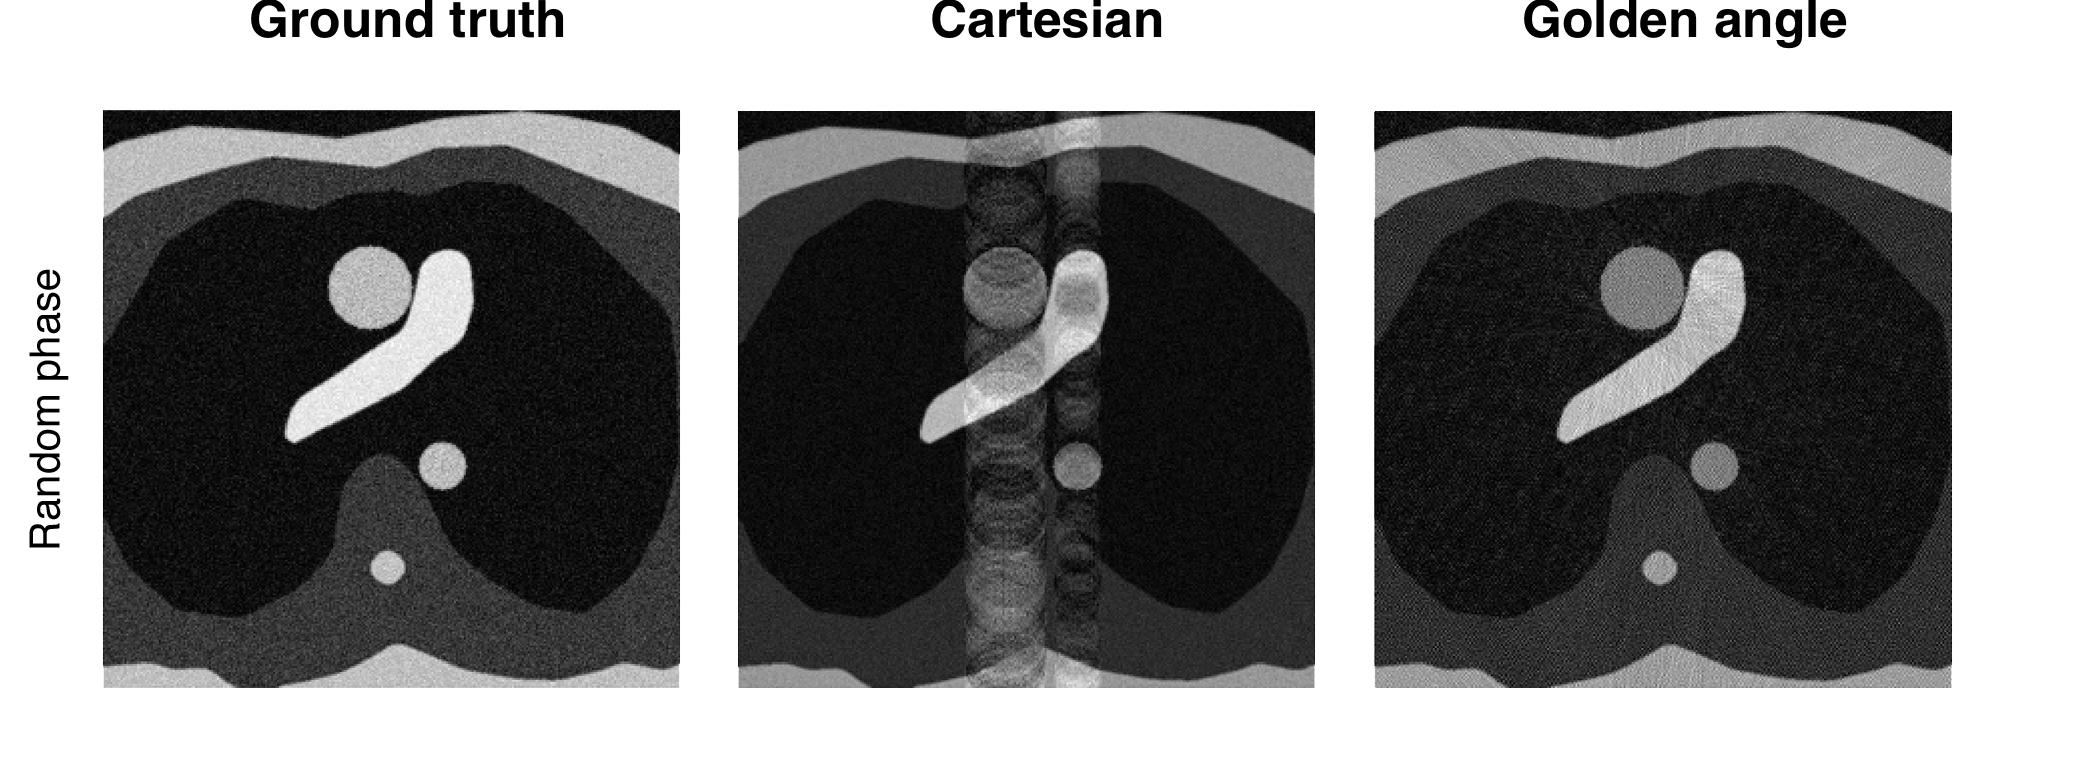
\includegraphics[width=\textwidth]{numerical.png}
    \caption{A numerical simulation of the effects of sampling an image with through-plane phase modulation when using a Cartesian (middle) and radial (left) readout trajectory. Reproduced with permission from~\cite{Fyrdahl2018}. Copyright \copyright~2018 International Society for Magnetic Resonance in Medicine. Published by John Wiley \& Sons Inc.}
    \label{fig:numerical}
\end{figure}
\subsect{Study II}
In Study II, a mathematical theory was proposed as a generalization for three-dimensional golden angles; see previous chapters. To evaluate the proposed generalization, numerical simulations were performed to calculate a clustered-regular-random (CRR) \Nomenclature{CRR}{Clustered Regular Random} value for the generalized profile orderings. CRR was defined as
\begin{equation}
    \textrm{CRR} = 2 \cdot \frac{\sum_{i\ne j}^{P} \textrm{min}(u_{i,j})}{\sqrt{P}}
\end{equation}
where P was the total number of sampling points and $u_{i,j}$ was the distance between sampling points $i$ and $j$. The mean angle between successive readout spokes was calculated as a measure of the gradient switching.

\subsect{Study III}
In Study III, numerical simulations of the point-spread function (PSF) \Nomenclature{PSF}{Point spread function} was performed. The PSF can be defined as the effect from voxel $i$ on all other voxels. The PSF due to voxel $i$ in voxel $j$ can be calculated as
\begin{equation}
    \textrm{PSF}(i,j) = e_j^*F^*e_i
    \label{eq:psf}
\end{equation}
where $e_i$ is a zero-vector with a single unitary value on the $i$th position and F is the encoding matrix, which in this case was the non-uniform Fourier operator.

The PSF was calculated for all voxels in an image frame, using the conventional golden-angle profile ordering and the proposed SWIG profile ordering. The maximum value and the sum-of-squares value of the PSF was calculated at concentric distances from the k-space center to classify the PSF at a distance from the k-space center.
\subsect{Study IV}
In Study IV, an extension of the profile ordering from Study III was proposed in 3D. The profile ordering was calculated for 12, 48 and 192 sectors, and the PSF was classified for each profile ordering, as described in Eq.~\ref{eq:psf}. Physiological binning was calculated for the 3 subjects, for both the conventional golden-angle profile ordering and the 3D-SWIG profile ordering, where 20 cardiac bins were calculated for each subject. Spherical Voronoi diagrams were calculated for each of the bins, and the mean Voronoi area was used as a metric of k-space uniformity.

\sect{Image acquisition and analysis}
All images were acquired on two clinical MRI systems from the vendor Siemens. One system had a field strength of 1.5 Tesla (Aera, Siemens Healthcare, Erlangen, Germany) and the other had a field strength of 3 Tesla (Skyra, Siemens Healthcare, Erlangen, Germany). The scanner software version on all scanners were the same for all studies included in this thesis (syngo MR E11A, Siemens Healthcare, Erlangen, Germany). The signal reception was performed with nearly identical surface coil arrays for both field strengths. One 18 channel general purpose ``body'' receive-only coil (Body 18, Siemens Healthcare, Erlangen, Germany) comprised of 3 rows with 6 coil elements on each row, giving a total of 18 coil array elements and a ``spine'' receive-only coil integrated into the patient table (Spine 32, Siemens Healthcare, Erlangen, Germany) comprising 8 rows with 4 coil elements on each row, giving a total of 32 coil array elements. Both systems were equipped with the same gradient specifications. The maximum gradient amplitude was 45 mT/m and the maximum slew rate was 200 T/m/s.
\subsect{Study I}
The protocol in Study I was designed to compare the novel proposed method to a previously proposed Cartesian protocol, using non-enhanced bSSFP and multiple repetitions of each slice position~\cite{Nyren2017}. Two image series were acquired, one golden-angle radial image series and one Cartesian image series. Both series comprised 70 contiguous slices with 3 mm slice thickness and no slice gap to cover the entire thorax. The sequences were matched as closely as possible, but due to technical limitations, some adjustment had to be made. All sequence parameters are outlined in Table~\ref{table:study1protocol}.
\begin{table}[htbp]
\caption{Sequence parameters from Study I.}
\begin{center}
\begin{threeparttable}
\begin{tabular}{l c c}
     \mydarkrowcolor \textbf{Parameter} & \textbf{Cartesian} & \textbf{Golden-Angle}\\
     TE (ms) & 1.6 & 1.8   \\
     \myrowcolor TR (ms) & 1.8 & 3.6 \\
     Readout lines (N)  & 163 & 1345 \\
     \myrowcolor Parallel imaging method & GRAPPA & SPIRiT \\
     ACS lines (N) & 38 & –– \\
     \myrowcolor Flip angle (deg) & 60 & 60 \\
     Bandwidth (Hz/px) & 1008 & 1008 \\
     \myrowcolor FOV (mm$^2$) & 420 & 420 \\
     Matrix size (px) & 288 & 288 \\
     \myrowcolor Acquired voxel size (mm$^2$) & $2\times2$ & $2\times2$\\
     Reconstructed voxel size (mm$^2$) & $2\times2$ & $2\times2$\\
     \myrowcolor Slice thickness (mm) & 3 & 3\\
    Number of slices (N) & 70 & 70 \\
    \myrowcolor Acq. time per slice (ms) & 522 & 4842 \\
    Total acq. time (s) & 40 & 340 \\
     \bottomrule
\end{tabular}
\begin{tablenotes}
\emph{Note:} ACS = Auto-calibrating signal \Nomenclature{ACS}{Auto-calibrating signal}.
\end{tablenotes}
\end{threeparttable}
\end{center}
\label{table:study1protocol}
\end{table}
From the golden-angle acquisitions, there where two additional data sets created by truncating the long acquisition. These corresponded to an oversampled set, an approximately fully sampled set and one undersampled set. The number of spokes in the oversampled set was chosen as all acquired spokes, the number of spokes in the fully sampled set was chosen as the Fibonacci number closest to a fully sampled acquisition according to the radial Nyquist criterion (i.e. the Nyquist criterion fulfilled at all parts of k-space) and the undersampled set was chosen such that the acquisition time matched that of the Cartesian acquisition. See Table~\ref{table:study1subgroups} for a complete description of the three data sets used for further analysis.
\begin{table}[htbp]
\caption{Description of the subgroups from Study I.}
\begin{center}
\begin{threeparttable}
\begin{tabular}{l c c c}
     \mydarkrowcolor \textbf{Parameter} & \textbf{Oversampled} & \textbf{Fully sampled} & \textbf{Undersampled}\\
     Spokes & 1345 & 610 & 144 \\
     \myrowcolor Cartesian undersampling (R) & 0.2 & 0.5 & 2 \\
     Radial undersampling & 0.33 & 0.74 & 3.1 \\
     \myrowcolor Acq. time per slice (ms) & 4842 & 2196 & 518 \\ 
     Total acq. time (s) & 340 & 150 & 40 \\
     \bottomrule
\end{tabular}
\begin{tablenotes}
\emph{Note:} Cartesian undersampling is the matrix size divided by the number of spokes. Radial undersampling is calculated relative to the Nyquist criterion at the edge of k-space.
\end{tablenotes}
\end{threeparttable}
\end{center}
\label{table:study1subgroups}
\end{table}
The previously described protocol was performed in 10 healthy volunteers, and in 2 patients. In one healthy volunteer, an additional acquisition was performed. In 20 slices covering the right pulmonary artery (RPA) and the left pulmonary artery (LPA). The acquisitions were performed during free-breathing, breath hold (end-expiratory), with ECG-triggering, and with a combination of breath hold and ECG-triggering.
In the patients, the blood-to-blood-clot contrast was measured by delineating blood clots and measuring the signal intensity within the clot. The blood-to-blood-clot-contrast was then calculated as
\begin{equation}
    C_{\textrm{blood,clot}} = \frac{S_{\textrm{blood}} - S_{\textrm{clot}}}{S_{\textrm{blood}}+S_{\textrm{clot}}}.
    \label{eq:bloodclotcontrast}
\end{equation}
The sharpness of pulmonary vessels was calculated using the Deriche algorithm~\cite{Deriche1990} by computing an edge image using a recursive Gaussian filter algorithm, then calculating a line-profile perpendicular to the vessels. The amplitude of the vessel wall in the edge image was used as a metric of the vessel sharpness.

Qualitative analysis of the images was performed using observer scoring, where two experienced radiologists were asked to score the images on a scale from 1 to 5, where a higher score signified better quality than a lower score.

\subsect{Study II}

A prototype 3D-radial bSSFP pulse sequence was modified to allow for sampling with 3D golden-angles. A user-selectable parameter was added to the sequence that allowed the operator to freely select a parameter that controlled the degree of the generalized profile ordering. By increasing the parameter, the mean angle between successive readouts was decreased. For further details on the implementation, see Study II.

Pre-recorded physiological signals (respiration and ECG) from 8 healthy volunteers were used to simulate physiological binning~\cite{Holst2017} and spherical Voronoi diagrams were calculated on the surface of the trajectory sphere. The standard deviation of the Voronoi cell area was used as a measure of the resultant sampling uniformity after the physiological binning was performed.

\subsect{Study III}
In Study III, a novel phase-contrast pulse sequence was proposed to enable high temporal resolution measurements of blood flow and tissue velocities.

In all subjects, a short-axis slice was planned by placing the imaging slice plane at the tip of the mitral valves in systole. Two images were acquired using this planning. One image with VENC = 30 cm/s for myocardial tissue velocities, and one image with VENC = 150 cm/s for transmitral blood flow velocities, see Figure~\ref{fig:swig_planning}.

\begin{figure}[htbp]
    \centering
    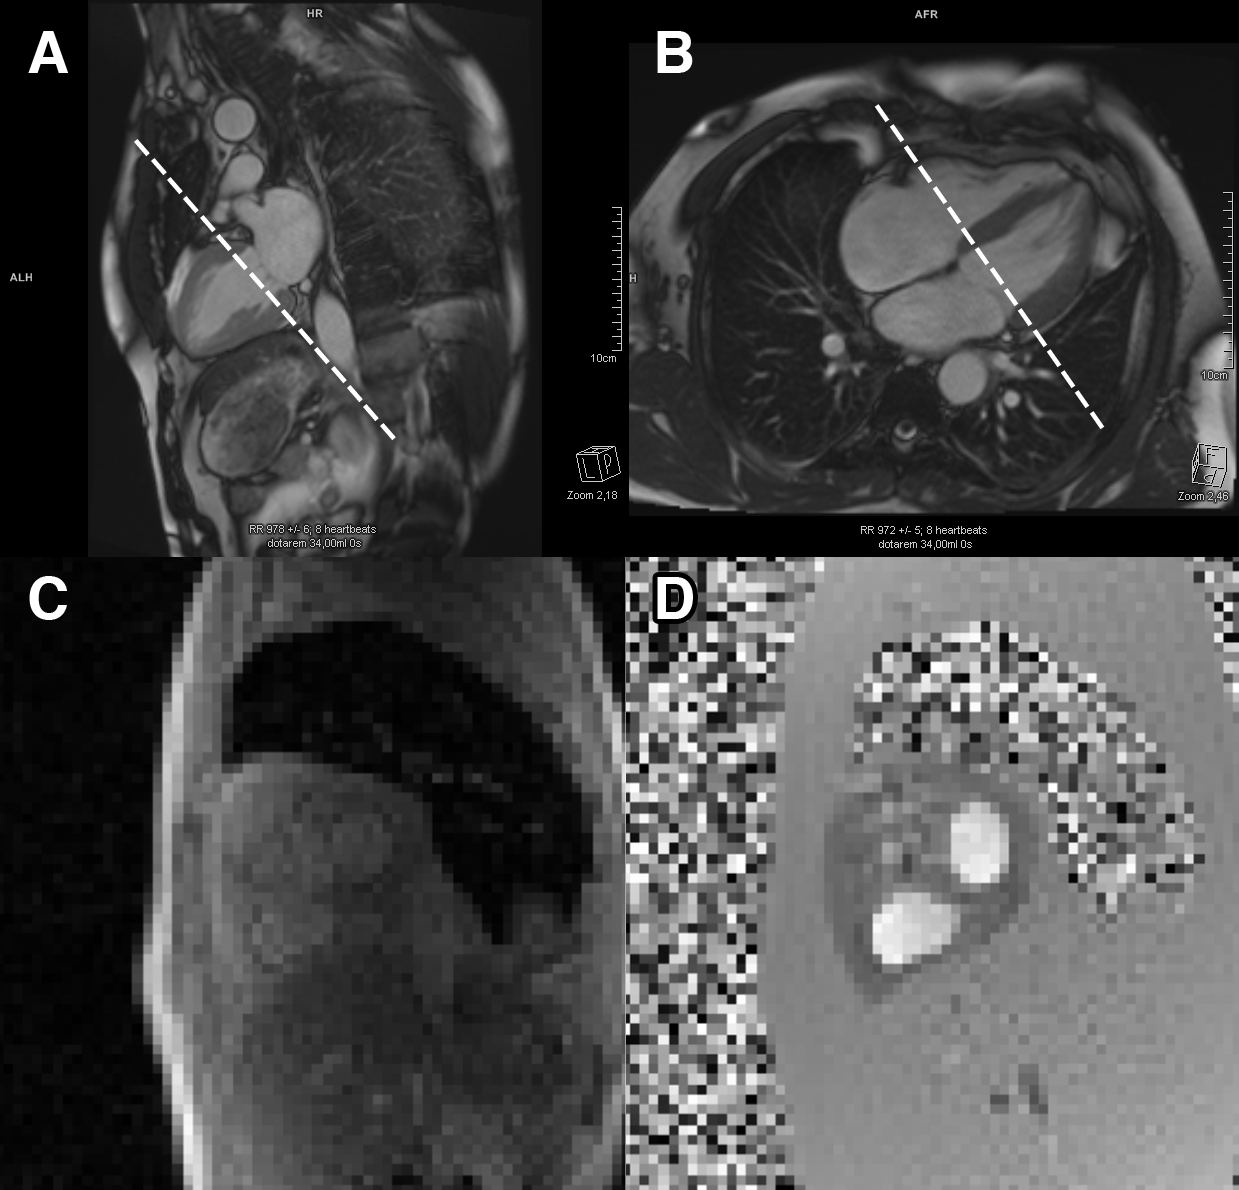
\includegraphics[width=0.75\textwidth]{Figure_2_planning.png}
    \caption{Planning was performed by planning a short-axis slice, indicated by the dashed white line, at the tip of the mitral leaflets in end-systole. The planning is displayed in a 2-chamber orientation (A) and a 4-chamber orientation (B). The resulting images from SWIG pulse sequences are displayed as a magnitude (C) and phase (D) image pair using VENC = 150 cm/s for transmitral blood flow measurements.}
    \label{fig:swig_planning}
\end{figure}

The image analysis was performed in Segment v2.1 R6069 (Medviso AB, Lund, Sweden)~\cite{Heiberg2010} using an in-house developed plugin to enable velocity measurements in a single voxel at the time, see Figure~\ref{fig:segment_gui}. Prior to analysis, quadratic static tissue compensation was performed, as well as semi-automatic phase unwrapping in the few cases where this was necessary.

\begin{figure}[htbp]
    \centering
    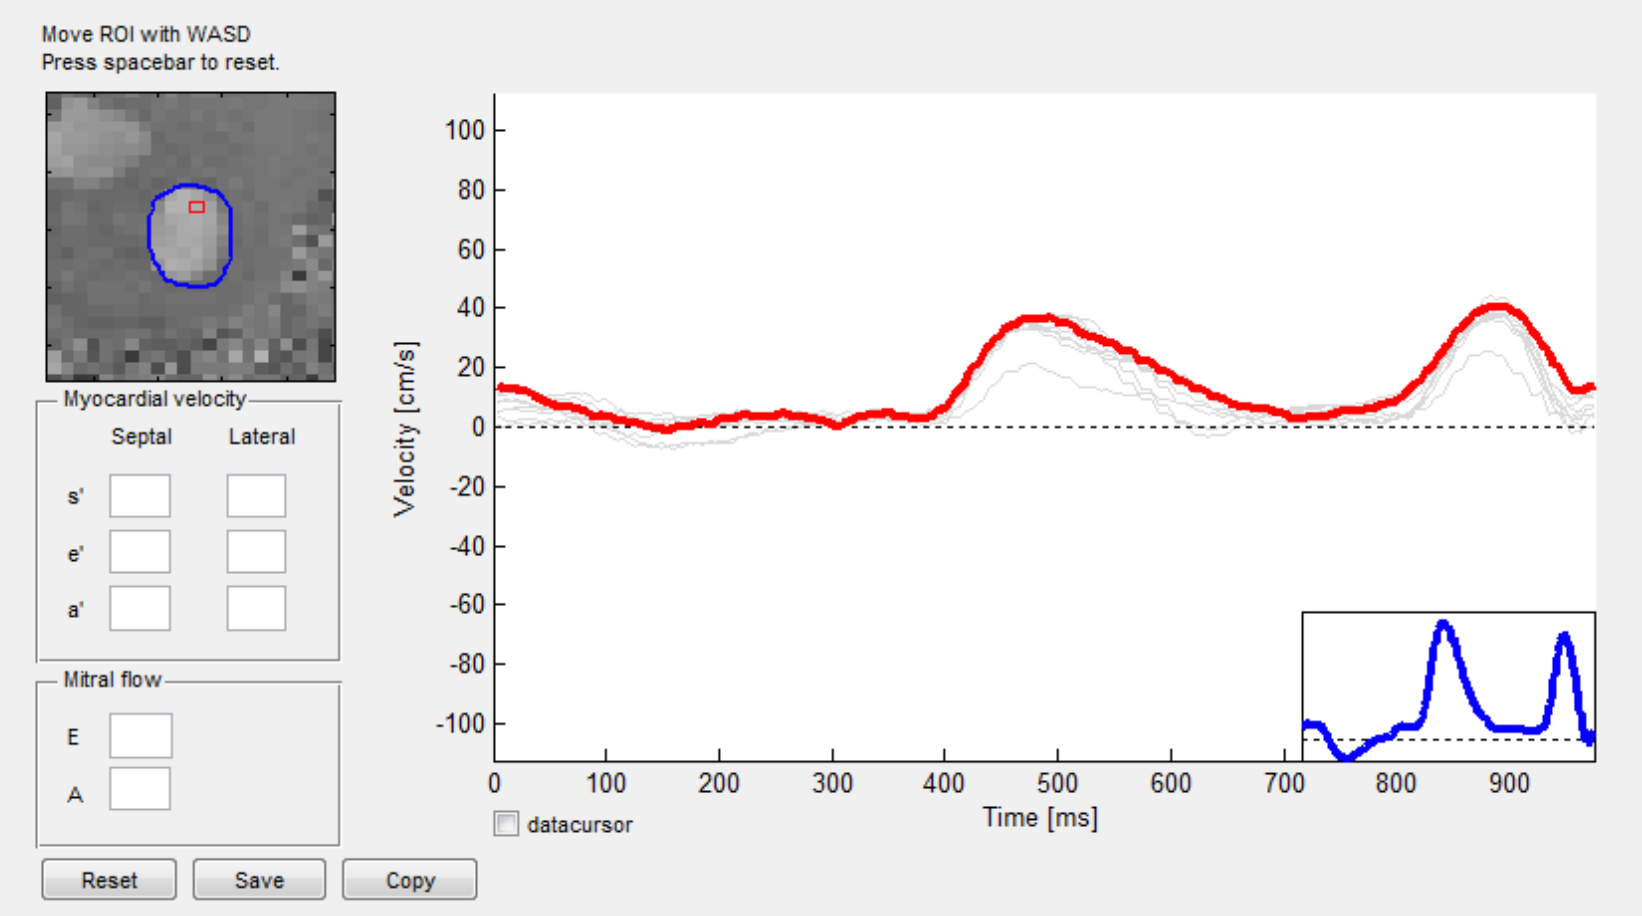
\includegraphics[width=\textwidth]{Figure_3_plugin.png}
    \caption{The measurement graphical user interface (GUI) was implemented as a plugin to the freely available image analysis software, Segment~\cite{Heiberg2010}. The image in the top left corner shows a cine loop of the phase image. The blue ROI indicates the manual identification of the mitral valve orifice, and the red square indicates the currently selected measurement voxel. The velocity in the selected measurement voxel is displayed as a red time-velocity curve in the main window. The average velocity within the blue ROI is displayed as a blue time-velocity curve in the inset window in the bottom right corner. The time-velocity curves in the adjacent (8-connected) voxels are displayed as light gray curves in the background.}
    \label{fig:segment_gui}
\end{figure}

The peak transmitral blood flow velocity was measured in the early filling (E) and late filling (A) phases, as well as the tissue velocity during systole (s'), during early filling (e') and during late filling (a'). The tissue velocities were measured in the lateral wall of the left ventricle and in the septum. Corresponding echocardiographic pulsed-wave Doppler and pulsed-wave tissue Doppler velocity measurements were measured using ViewPoint (GE Healthcare, Chicago, IL).

\subsect{Study IV}
A prototype 3D radial bSSFP pulse sequence was modified to allow for sampling with the 3D-SWIG profile ordering. For further details on the implementation, see Study II. Phantom acquisitions were performed using the conventional double golden-angle profile ordering and one acquisition using the 3D-SWIG profile ordering, using 12, 48 and 192 sectors. For the patients, one acquisition using the conventional double golden-angle profile ordering and one acquisition using the 3D-SWIG profile ordering, using 48 sectors, were acquired in all three subjects. Relevant sequence parameters were TE = 1.7 ms, TR = 3.4 ms, flip angle = $50^\circ$, voxel size 1.2 mm isotropic, for both acquisitions.